\documentclass[12pt,a4paper]{article}
\usepackage[left=25mm,right=20mm,top=20mm,bottom=20mm]{geometry}
\usepackage{url}
\usepackage{graphicx}
\usepackage[utf8]{vietnam}
\usepackage{circuitikz}
\usepackage{physics}
\usetikzlibrary{calc,positioning}
\usepackage{caption,subcaption}
\usepackage{amsfonts,amsmath}
\usepackage{derivative}
\usepackage{indentfirst}
\setlength{\parindent}{1cm}
\usepackage{tabularx}
\newcolumntype{Y}{>{\small\centering\arraybackslash}X}
\usepackage{enumitem}
\usepackage{pdflscape}
\usepackage{listings}
\usepackage{xcolor}

% Định nghĩa style cho MATLAB
\lstdefinestyle{matlabstyle}{
    language=Matlab,
    basicstyle=\ttfamily\small,       % Font code
    keywordstyle=\color{blue},        % Từ khóa màu xanh
    commentstyle=\color{green!50!black}, % Comment màu xanh lá đậm
    stringstyle=\color{orange},       % Chuỗi màu cam
    numbers=left,                     % Đánh số dòng bên trái
    numberstyle=\tiny\color{gray},    % Màu số dòng
    stepnumber=1,                     % Số dòng cách nhau 1
    numbersep=8pt,                    % Khoảng cách số dòng và code
    backgroundcolor=\color{gray!5},   % Nền xám nhạt
    showspaces=false,                 
    showstringspaces=false,
    showtabs=false,                   
    frame=single,                     % Khung viền
    tabsize=4,                        
    breaklines=true,                  % Tự xuống dòng
    breakatwhitespace=false,
    escapeinside={\%*}{*)}            % Chèn code LaTeX trong code
}
\begin{document}
\everymath{\displaystyle}
\begin{titlepage}
    \begin{tikzpicture}[remember picture,overlay,inner sep=0,outer sep=0]
     \draw[blue!70!black,line width=4pt] ([xshift=-1.5cm,yshift=-2cm]current page.north east) coordinate (A)--([xshift=1.5cm,yshift=-2cm]current page.north west) coordinate(B)--([xshift=1.5cm,yshift=2cm]current page.south west) coordinate (C)--([xshift=-1.5cm,yshift=2cm]current page.south east) coordinate(D)--cycle;

     \draw ([yshift=0.5cm,xshift=-0.5cm]A)-- ([yshift=0.5cm,xshift=0.5cm]B)--
     ([yshift=-0.5cm,xshift=0.5cm]B) --([yshift=-0.5cm,xshift=-0.5cm]B)--([yshift=0.5cm,xshift=-0.5cm]C)--([yshift=0.5cm,xshift=0.5cm]C)--([yshift=-0.5cm,xshift=0.5cm]C)-- ([yshift=-0.5cm,xshift=-0.5cm]D)--([yshift=0.5cm,xshift=-0.5cm]D)--([yshift=0.5cm,xshift=0.5cm]D)--([yshift=-0.5cm,xshift=0.5cm]A)--([yshift=-0.5cm,xshift=-0.5cm]A)--([yshift=0.5cm,xshift=-0.5cm]A);


     \draw ([yshift=-0.3cm,xshift=0.3cm]A)-- ([yshift=-0.3cm,xshift=-0.3cm]B)--
     ([yshift=0.3cm,xshift=-0.3cm]B) --([yshift=0.3cm,xshift=0.3cm]B)--([yshift=-0.3cm,xshift=0.3cm]C)--([yshift=-0.3cm,xshift=-0.3cm]C)--([yshift=0.3cm,xshift=-0.3cm]C)-- ([yshift=0.3cm,xshift=0.3cm]D)--([yshift=-0.3cm,xshift=0.3cm]D)--([yshift=-0.3cm,xshift=-0.3cm]D)--([yshift=0.3cm,xshift=-0.3cm]A)--([yshift=0.3cm,xshift=0.3cm]A)--([yshift=-0.3cm,xshift=0.3cm]A);

   \end{tikzpicture}

\begin{center}
    {\bfseries\large
        ĐẠI HỌC QUỐC GIA THÀNH PHỐ HỒ CHÍ MINH

        TRƯỜNG ĐẠI HỌC BÁCH KHOA

    }

    \vspace{\baselineskip}

    {\large
        KHOA CƠ KHÍ
        
        BỘ MÔN CƠ ĐIỆN TỬ
    }

    \vspace{3\baselineskip}

    
\includegraphics[scale=4]{logo_bk.pdf}

    \vspace{2\baselineskip}

    {\LARGE Bài tập lớn}

    \vspace{0.5\baselineskip}
    
    \textbf{\LARGE Động lực học và Điều khiển (ME3011)}

    
    \vfill

    \begin{tabular}{ll}
        \textit{Giảng viên hướng dẫn} &  TS. Phạm Phương Tùng\\
        \textit{Lớp} & DT01\\
        \textit{Thành viên nhóm} & 
    \end{tabular}

    \begin{tabularx}{0.75\linewidth}{|X|c|c|}
        \hline
        \multicolumn{1}{|c|}{\textbf{\textbf{Họ và tên}}} & \textbf{MSSV} & \multicolumn{1}{c|}{\textbf{Nhiệm vụ chính}}\\ \hline
        Nguyễn Đức Đạt & 211100\textcolor{red}{9} & \\ \hline
        Trần Quang Đạo & 221064\textcolor{red}{7} & \\ \hline
        Thành viên bí mật & XXXXXX\textcolor{red}{2} & Cung cấp chữ số cuối MSSV\\ \hline
    \end{tabularx}

    \vspace{3\baselineskip}

    \textbf{TP.HCM, 22/08/2025}
    \vspace{\baselineskip}
\end{center}
\end{titlepage}

\newpage

\tableofcontents
\newpage

\section{Tổng quan}
Bài tập lớn tập trung vào việc mô hình hóa động lực học và điều khiển cần cẩu tháp. Hệ thống 
có thể mô hình hóa đơn giản như hệ thống con lắc gắn trên xe đẩy. Sinh viên sẽ xây dựng mô 
hình, thiết kế bộ điều khiển và thực hiện mô phỏng để đạt được các yêu cầu về ổn định con lắc 
và vị trí xe đẩy.  

Với hệ thống con lắc trên xe đẩy, giả sử các thông số sau: 

\begin{table}[ht]
    \centering
    \begin{tabular}{|l|l|}
        \hline
        \multicolumn{1}{|c|}{\textbf{Thông số}} & \multicolumn{1}{c|}{\textbf{Giá trị}} \\ \hline
        \rule{0pt}{7mm}Khối lượng của xe đẩy $m_1$ & $\frac{9+7+2}{10} = 1.8$ kg\\[3mm] \hline
        \rule{0pt}{7mm}Khối lượng của con lắc $m_2$ & $\frac{2+7}{20} = 0.45$ kg \\[3mm] \hline
        \rule{0pt}{7mm}Chiều dài dây cáp $L$ & $\frac{7+2}{20} = 0.45$ m \\[3mm] \hline
        \rule{0pt}{7mm}Hệ số ma sát của xe đẩy $B$ &  $\frac{9+2}{10\times 7} =0.15714 $ Ns/m\\[3mm] \hline
        \rule{0pt}{7mm}Hệ số tắt dần của con lắc $b$ & $\frac{9+7}{10\times 2} = 0.8$ Ns/m \\[3mm] \hline 
    \end{tabular}
    \caption{Bảng thông số hệ thống}
\end{table}

\newpage
\section{Mô hình hóa}

\subsection{Phân tích lực và xây dựng phương trình vi phân mô tả hệ}

Hệ thống con lắc và xe đẩy có sơ đồ như sau:
\begin{figure}[ht]
    \centering
    \begin{circuitikz}[x=1mm,y=1mm]
        \node[draw,minimum width=1.5cm,minimum height=1cm] (m1) at (0,0) {$m_1$};
        \node[draw,minimum size=0.5cm, circle,fill=black,inner sep=0pt] (m2) at ($(m1.-90)+(-120:40)$) {}; 
        \draw (m2) -- (m1.-90) node[midway,left] {$L$};
        \draw[dashed] (m1.-90) -- ++(0,-25);
        \draw[latex-latex] (m1.-90) ++ (-90:10) arc (-90:-120:10) node[below,midway] {$\theta$};
        \fill[black!20] (m1.-90)++(-35,5) rectangle ++(-2.5,-10);
        \draw[very thick] (m1.-90)++(-35,5) --++(0,-10);
        \draw[very thick] (m1.-90)++(-35,0) -- ++(70,0);
        \draw[latex-,very thick] (m1.180) -- ++(-15,0) node[left] {$F$};
        \node[below] at (m2.-90) {$m_2$};
    \end{circuitikz}
    \caption{Sơ đồ hệ con lắc và xe đẩy}
    \label{fig:1}
\end{figure}

Gọi $\vb r_x$ và $\vb r_c$ lần lượt là vector vị trí của xe và con lắc đơn. Ta sẽ biểu diễn $\vb r_x$ và $\vb r_c$ theo 2 vector đơn vị $\vb{\hat i}$ và $\vb{\hat j}$ dựa vào hình dưới như sau:
\begin{equation}
    \begin{aligned}
    \vb r_x  &= x \vb{\hat i} + 0\vb{\hat j}\\
    \vb r_c  &= (x - L\sin\theta)\vb{\hat i} -L\cos\theta \vb{\hat j}
\end{aligned}
\end{equation}


\begin{figure}[ht]
    \centering
    \begin{circuitikz}[x=1mm,y=1mm]
        \node[draw,minimum width=1.5cm,minimum height=1cm] (m1) at (0,0) {$m_1$};
        \node[draw,minimum size=0.5cm, circle,fill=black,inner sep=0pt] (m2) at ($(m1.-90)+(-120:40)$) {}; 
        \draw (m2) -- (m1.-90) node[midway,left] {$L$};
        \draw[dashed] (m1.-90) -- ++(0,-55);
        \draw[latex-latex] (m1.-90) ++ (-90:10) arc (-90:-120:10) node[below,midway] {$\theta$};
        \draw[very thick,-latex] (m1.-90)++(-35,-50) -- ++(35,0) node[above,midway] {$\vb r_x=x \vb{\hat i} + 0\vb{\hat j}$};
        \draw[very thick,-latex] (m1.-90)++(-35,0) -- (m2) node[right,midway] {$\vb r_c$};
        \fill ($(m1.-90)+(-35,0)$) circle (1);
        \node[right] at (m2.0) {$m_2$};
        \draw[very thick,-latex] (m1.-90) ++ (-35,0) -- ++(15,0) node[right] {$\vb{\hat i}$};
        \draw[very thick,-latex] (m1.-90) ++ (-35,0) -- ++(0,15) node[above] {$\vb{\hat j}$};
        \draw (m1.-90) ++ (-35,0) -- ++(0,-55);
    \end{circuitikz}
    \caption{Biểu diễn vector vị trí theo hai vector $\vb{\hat i}$ và $\vb{\hat j}$}
    \label{fig:2}
\end{figure}

Đạo hàm theo thời gian hai vector $\vb r_x$ và $\vb r_c$ ta có:
\begin{equation}
    \begin{aligned}
    \vb{\dot r_x}  &= \dot x \vb{\hat i} + 0\vb{\hat j}\\
    \vb{\dot r_c}  &= (\dot x - L\dot\theta \cos\theta)\vb{\hat i} +L\dot\theta\sin\theta \vb{\hat j}
\end{aligned}
\end{equation}

Tiếp tục đạo hàm theo thời gian hai vector $\vb {\dot r_x}$ và $\vb {\dot r_c}$ để thu được hai vector gia tốc:
{\small
\begin{equation}
    \begin{aligned}
    \vb{\ddot r_x}  & = \ddot x \vb{\hat i} + 0\vb{\hat j}\\
    \vb{\ddot r_c}  & = (\ddot x + L\dot\theta^2 \sin\theta - L\ddot \theta cos\theta)\vb{\hat i} +(L\dot\theta^2\cos\theta + L \ddot\theta \sin\theta)\vb{\hat j} = \ddot x\vb{\hat i} + L \dot\theta^2 (\sin\theta \vb{\hat i}+\cos\theta \vb{\hat j}) + L\ddot\theta (-\cos \theta\vb{\hat i} +\sin\theta\vb{\hat j}) \label{eqn:r}
\end{aligned}
\end{equation}}

Hệ có 2 bậc tự do là $x$ và $\theta$ nên hệ sẽ có hai phương trình mô tả chuyển động, gồm một phương trình chuyển động tịnh tiến của xe đẩy và một phương trình chuyển động quay của con lắc.

Từ sơ đồ tổng thể trong hình \ref{fig:1} và \ref{fig:2}, ta tách thành hai sơ đồ vật tự do (free body diagram) để phân tích lực tác dụng lên từng thành phần của hệ dựa vào các gia tốc mà ở phương trình \eqref{eqn:r}.
\begin{figure}[ht]
    \centering
    \begin{subfigure}[b]{0.49\linewidth}
        \centering
        \begin{circuitikz}[x=1mm,y=1mm]
            \node[draw,minimum width=1.5cm,minimum height=1cm] (m1) at (0,0) {$m_1$};
            \draw[latex-,very thick] (m1.180) -- ++(-15,0) node[left] {$F$};
            \draw[-latex,very thick] (m1.-90) -- ++(-120:15) node[below left] {$R$};  
            \draw[latex-,very thick] (m1.90)++(-4,0) -- ++(0,15) node[above] {$m_1g$};
            \draw[latex-,very thick] (m1.0) ++ (0,2.5) -- ++(15,0) node[right] {$B\dot x$};
            \draw[-latex,very thick,dashed] (m1.0) ++(0,-2.5) -- ++(15,0) node[right] {$\ddot x$};
            \draw[dashed] (m1.-90) -- ++(0,-25);
            \draw[latex-latex] (m1.-90) ++ (-90:10) arc (-90:-120:10) node[below,midway]{$\theta$};
            \draw[-latex,very thick] (m1.90) ++(4,0) --++(0,15) node[above] {$N$};
        \end{circuitikz}
        \caption{Xe đẩy}
    \end{subfigure}\hfill
    \begin{subfigure}[b]{0.49\linewidth}
        \centering
        \begin{circuitikz}[x=1mm,y=1mm]
            \node[draw,minimum size=0.5cm, circle,fill=black,inner sep=0pt] (m2) at ($(0,0)+(-120:40)$) {}; 
            \draw (m2) -- (0,0) node[near end,left] {$L$};
            \draw[dashed] (0,0) --++(0,-25);
            \draw[latex-latex] (0,0) ++ (-90:10) arc (-90:-120:10) node[below,midway] {$\theta$};
            \node[left] at (m2.180) {$m_2$};
            \draw[-latex,very thick] (m2.-90) --++(0,-15) node[below] {$m_2g$};
            \draw[-latex,very thick] (0,0) --++(60:15) node[above] {$R$};
            \draw[-latex,dashed,very thick] (m2.60) -- ++(60:15) node[right,midway] {$L\dot\theta^2$};
            \draw[-latex,dashed,very thick] (m2.150) -- ++(150:15) node[left] {$L\ddot\theta$};
            \draw[-latex,dashed,very thick] (m2.0) --++ (15,0) node[right] {$\ddot x$};
            \draw[-latex,very thick] (0,0) ++(200:20) arc (200:280:20) node[left,very near start] {$b\dot\theta$};
            %\draw[-latex,very thick] (0,0)++(180:5) arc (180:-60:5) node[above, midway] {$b\dot\theta$};
        \end{circuitikz}
        \caption{Con lắc}
    \end{subfigure}
    \caption{Sơ đồ vật tự do của con lắc và xe đẩy với $R$ là phản lực tác dụng từ con lắc lên xe đẩy. Phương, chiều của các gia tốc (nét đứt) được xác định dựa trên phương trình \eqref{eqn:r}}
\end{figure}


\textbf{Với xe đẩy}, theo định luật II Newton, ta có:
\begin{align}
    m_1\ddot x = F- B\dot x - R\sin\theta \label{eqn:1}
\end{align}

\textbf{Với con lắc}, theo định luật II Newton, ta có:
\begin{align}
    m_2(\ddot x - L\ddot\theta\cos\theta +  L\dot\theta^2\sin\theta ) = R\sin\theta \label{eqn:2}
\end{align}

Ngoài ra, theo định luật II Newton cho hệ quay quanh tâm quay con lắc , ta có:
\begin{align}
    m_2L (L \ddot\theta -\ddot x\cos\theta) =- m_2Lg\sin\theta -b\dot\theta\label{eqn:3}
\end{align}

Kết hợp các phương trình \eqref{eqn:1}, \eqref{eqn:2} và \eqref{eqn:3}, thu được
\begin{equation}
    \begin{aligned}
        (m_1 + m_2)\ddot x + B\dot x - m_2L\ddot\theta\cos\theta + m_2L\dot\theta^2 \sin\theta = F\\
     m_2L^2 \ddot\theta + b\dot\theta + m_2Lg\sin\theta - m_2L\ddot x \cos\theta = 0
    \end{aligned}\label{eqn:4}
\end{equation}

\subsection{Tuyến tính hóa hệ thống và xây dựng hàm truyền}

Khi góc $\theta$ trở nên rất nhỏ ($\theta\to 0$), ta có thể xấp xỉ $\sin \theta \approx \theta,\cos\theta \approx 1$ và $\dot\theta^2 \approx 0$. Do đó, ta có thể tuyến tính hóa hệ phương trình \eqref{eqn:4} như sau:
\begin{equation}
    \begin{aligned}
        (m_1 + m_2)\ddot x + B\dot x - m_2L\ddot\theta  = F\\
     m_2L^2 \ddot\theta + b\dot\theta + m_2Lg\theta - m_2L\ddot x  = 0
    \end{aligned}\label{eqn:5}
\end{equation}

Biến đổi Laplace hệ phương trình \eqref{eqn:5} với điều kiện đầu bằng không, ta có:
\begin{equation}
    \begin{aligned}
        \lbrack(m_1+m_2)s^2 + Bs\rbrack X(s) - m_2 Ls^2 \Theta(s) = F(s)\\
        -m_2 L s^2 X(s) + (m_2L^2s^2 + bs + m_2Lg)\Theta(s) = 0
    \end{aligned}\label{eqn:6}
\end{equation}

Giải hệ phương trình \eqref{eqn:6} thu được các hàm truyền:
\begin{enumerate}
    \item Thể hiện mối quan hệ giữa vị trí xe đẩy và lực đầu vào
    {\footnotesize	
    \begin{align}
        G_1(s)=\frac{X(s)}{F(s)} = \frac{m_2L^2s^2 + bs + m_2Lg}{m_1 m_2 L^2 s^4 + [(m_1 + m_2)b + B m_2 L^2] s^3 + [(m_1 + m_2)m_2 g L + B b] s^2 + B m_2 g L s}
    \end{align}}
    \item Thể hiện mối quan hệ giữa góc lắc và lực đầu vào
    {\footnotesize	
    \begin{align}
        G_2(s)=\frac{\Theta(s)}{F(s)} = \frac{m_2Ls}{m_1 m_2 L^2 s^3 + [(m_1 + m_2)b + B m_2 L^2] s^2 + [(m_1 + m_2)m_2 g L + B b] s + B m_2 g L}
    \end{align}}
\end{enumerate}

\subsection{Phương trình không gian trạng thái của hệ}
Giải hệ phương trình \eqref{eqn:5} theo hai biến $\ddot x$ và $\ddot \theta$, ta thu được:
\begin{align}
    \ddot x & = -\frac{B\dot x}{m_1} - \frac{m_2g\theta}{m_1} - \frac{b\dot\theta}{m_1L} + \frac{F}{m_1}\label{eqn:9}\\
    \ddot \theta & = -\frac{B\dot x}{m_1 L} - \frac{(m_1+m_2)g\theta}{m_1L} - \frac{(m_1+m_2)b\dot\theta}{m_1m_2L^2}+ \frac{F}{m_1L} \label{eqn:10}
\end{align}

Chọn các biến $\vb x = \begin{bmatrix}
    x & \dot x & \theta & \dot\theta 
\end{bmatrix}^T$ làm biến trạng thái. Kết hợp với hai phương trình \eqref{eqn:9} và \eqref{eqn:5}, ta có phương trình trạng thái của hệ với đầu ra là $x$ và $\theta$:
\begin{align}
    \begin{bmatrix}
        \dot x \\ \ddot x \\ \dot \theta \\ \ddot\theta 
    \end{bmatrix} & = \begin{bmatrix}
        0 & 1 & 0 & 0 \\
        0 & -\frac{B}{m_1} & -\frac{m_2g}{m_1} & -\frac{b}{m_1L}\\
        0 & 0 & 0 & 1 \\
        0 & -\frac{B}{m_1L} & -\frac{(m_1+m_2)g}{m_1L} & -\frac{(m_1+m_2)b}{m_1m_2L^2}
    \end{bmatrix}\begin{bmatrix}
        x \\ \dot x \\ \theta \\ \dot\theta 
    \end{bmatrix} + \begin{bmatrix}
        0 \\ \frac{1}{m_1} \\ 0 \\ \frac{1}{m_1L}
    \end{bmatrix}F\label{eqn:11}\\
    \vb y & = \begin{bmatrix}
        1 & 0 & 0 & 0\\
        0 & 0 & 1 & 0
    \end{bmatrix}\begin{bmatrix}
        x \\ \dot x \\ \theta \\ \dot\theta 
    \end{bmatrix}\label{eqn:12}
\end{align}

\newpage
\subsection{Sơ đồ khối của không gian trạng thái}
Từ hệ phương trình trạng thái \eqref{eqn:11} và \eqref{eqn:12}, ta xây dựng được sơ đồ khối như sau:
\begin{figure}[ht]
    \centering
    \begin{circuitikz}[x=1mm,y=1mm,thick]
        \node[mixer,scale=0.75,thin] (m1) at (0,0) {};
        \node[right=15 of m1,draw, minimum width=2.5cm,minimum height=1cm] (tp1) {$\frac{1}{s}$};
        \node[right=20 of tp1,draw, minimum width=2.5cm,minimum height=1cm] (tp2) {$\frac{1}{s}$};

        \draw[-latex] (m1) -- (tp1) node[above,midway] {$\ddot x$};
        \draw[-latex] (tp1) -- (tp2) node[above,midway] {$\dot x$};
        \draw[-latex] (tp2.0) -- ++(15,0) node[above,midway] {$x$};

        \node[below=5 of tp1,draw, minimum width=2.5cm,minimum height=1cm] (x1) {$\frac{B}{m_1}$};
        \node[below=5 of x1,draw, minimum width=2.5cm,minimum height=1cm] (theta1) {$\frac{m_2g}{m_1}$};
        \node[below=5 of theta1,draw, minimum width=2.5cm,minimum height=1cm] (theta2) {$\frac{b}{m_1L}$};

        \draw[-latex] (tp1.0)++(7,0) |- (x1);
        \draw[-latex] (x1.180) -- ++(-5,0) -- (m1) node[near end,right=-1mm] {$-$};
        \draw[-latex] (theta1.180) -- ++(-10,0) -- (m1) node[near end,right=-1mm] {$-$};
        \draw[-latex] (theta2.180) -| (m1) node[very near end,left=-1mm] {$-$};

        \node[below=5 of theta2,draw, minimum width=2.5cm,minimum height=1cm] (theta3) {$\frac{(m_1+m_2)b}{m_1m_2L^2}$};
        \node[below=5 of theta3,draw, minimum width=2.5cm,minimum height=1cm] (theta4) {$\frac{(m_1+m_2)g}{m_1L}$};
        \node[below=5 of theta4,draw, minimum width=2.5cm,minimum height=1cm] (x2) {$\frac{B}{m_1L}$};

        \node[below=5 of x2,draw, minimum width=2.5cm,minimum height=1cm] (tp3) {$\frac{1}{s}$};
        \node[mixer,scale=0.75,left=15 of tp3,thin] (m2) {};
        \node[right=20 of tp3,draw, minimum width=2.5cm,minimum height=1cm] (tp4) {$\frac{1}{s}$};

        \draw[-latex] (m2) -- (tp3) node[below,midway] {$\ddot\theta$};
        \draw[-latex] (tp3) -- (tp4) node[below,midway] {$\dot\theta$};
        \draw[-latex] (tp4.0) -- ++(15,0) node[below,midway] {$\theta$};

        \draw[-latex] (tp1.0) ++(7,0) |- (x2);
        \draw[-latex] (x2.180) --++(-5,0) -- (m2) node[right=-1mm,near end] {$-$};
        \draw[-latex] (theta4.180) --++(-10,0) -- (m2) node[right=-1mm,near end] {$-$};
        \draw[-latex] (theta3) -| (m2) node[left=-1mm, very near end] {$-$};

        \foreach \x\y in {jctheta1/theta1,jctheta2/theta2,jctheta3/theta3,jctheta4/theta4}
        {
            \node[jump crossing,scale=2] (\x) at ($(\y.0) + (7,0)$) {};
            \draw[-latex] (\x.west) -- (\y);
        }
        \node[jump crossing, scale=2] (jctheta44) at ($(theta4.0) + (14,0)$) {};

        \draw (tp3.0) ++(14,0) |- (jctheta2.east) (tp3.0) ++(14,0) |- (jctheta3.east);
        \draw (tp4.0) ++(7.5,0) |- (jctheta1.east) (tp4.0) ++(7.5,0) |- (jctheta44.east);
        \draw (jctheta44.west) -- (jctheta4.east);
    
        \node[left=10 of m1,draw, minimum width=2.5cm,minimum height=1cm] (F1) {$\frac{1}{m_1}$};
        \node[left=10 of m2,draw, minimum width=2.5cm,minimum height=1cm] (F2) {$\frac{1}{m_1L}$};

        \draw[latex-] (F1.180) -- ++(-15,0) node[above,midway] {$F$};
        \draw[-latex] (F1.180) ++ (-7.5,0) |- (F2);
        \draw[-latex] (F1) -- (m1) node[above,near end] {$+$};
        \draw[-latex] (F2) -- (m2) node[above,near end] {$+$};
    \end{circuitikz}
    \caption{Sơ đồ khối của hệ thống xe đẩy-con lắc}
    \label{fig:4}
\end{figure}


\section{Phân tích hệ thống}

\subsection{Yêu cầu đề bài}
Mô phỏng đáp ứng hệ thống sử dụng mô hình sơ đồ khối trên MATLAB/Simulink. Phân tích 
và đánh giá đáp ứng hệ thống
\begin{enumerate}
    \item Với đầu vào $F(t)$ là hàm xung diract (impulse).
    \item Với đầu vào $F(t)$ là hàm nấc đơn vị (unit step). 
    \item Với đầu vào là như sau:
    \begin{align}
        F(t) = \begin{cases}
        10\ \text{N}, 0 \le t < 5\ \text{giây}\\
        0\ \text{N}, t \ge 5\ \text{giây}
    \end{cases} \label{eqn:hxd}
    \end{align}
\end{enumerate}

\subsection{Sơ đồ MATLAB/Simulink}

Dựa vào sơ đồ khối ở hình \ref{fig:4}, ta xây dựng được sơ đồ MATLAB/Simulink được cho như hình dưới: 

\begin{landscape}

\begin{figure}[ht]
    \centering
    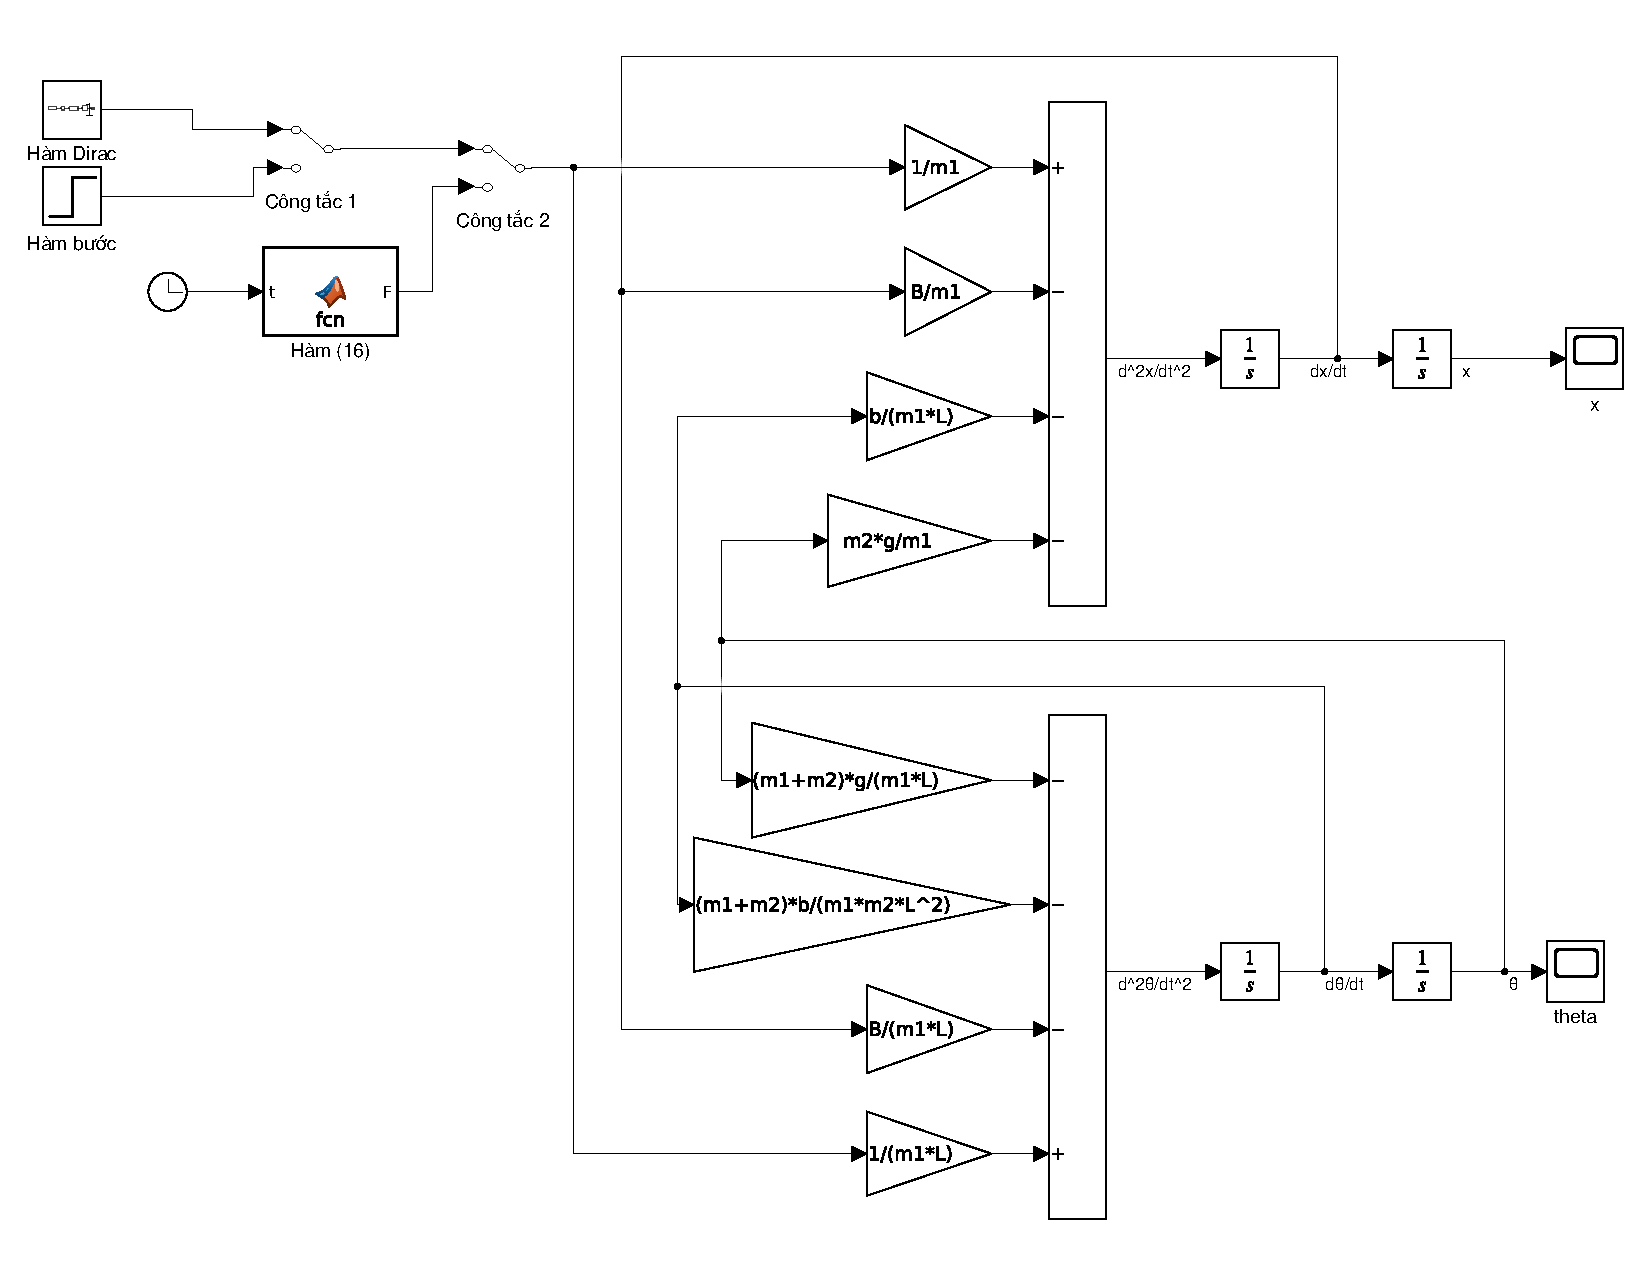
\includegraphics[height=0.5\paperheight]{MATLAB_1.pdf}
    \caption{Sơ đồ MATLAB/Simulink để phân tích hệ thống}
    \label{fig:m1}
\end{figure}
\end{landscape}

Trong sơ đồ MATLAB/Simulink hình \ref{fig:m1}, các hàm $F(t)$ đầu vào được khai báo như sau:
\begin{enumerate}
    \item Hàm Dirac được khai báo bằng khối \textbf{Hàm Dirac}. Khối này là một hệ con (subsystem) được xây dựng dựa vào một bài blog của MATLAB tại địa chỉ \url{https://tinyurl.com/yrh28h2j}.
    \begin{figure}[ht]
        \centering
        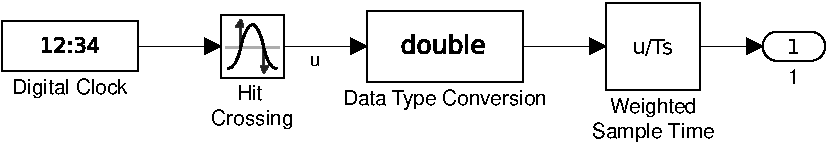
\includegraphics[width=\linewidth]{MATLAB_2.pdf}
        \caption{Nội dung khối \textbf{Hàm Dirac}}
    \end{figure}

    \item Hàm nấc đơn vị, sử dụng khối \textbf{Step} được khai báo như hình dưới
    \vspace{-5mm}
    \begin{figure}[ht]
        \centering
        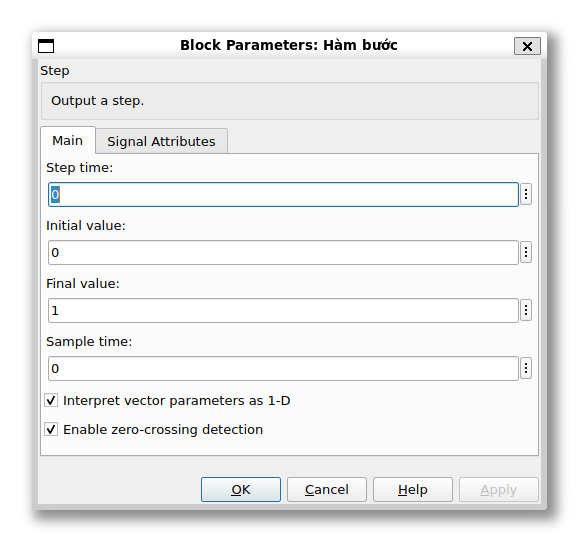
\includegraphics[width=0.5\linewidth]{MATLAB_3.png}
        \vspace{-5mm}
        \caption{Khai báo khối \textbf{Step} đối với hàm nấc đơn vị}
    \end{figure}

    \item Đối với hàm \eqref{eqn:hxd}, ta xây dựng bằng hàm \textbf{MATLAB function} như sau:
    \begin{lstlisting}[style=matlabstyle,caption=Khai báo hàm \eqref{eqn:hxd}]
function F = fcn(t)
    if t >= 0 && t <= 5
        F = 10;
    else
        F = 0;
    end
end        
    \end{lstlisting}
\end{enumerate}

\newpage
\subsection{Phân tích và đánh giá kết quả mô phỏng}
\subsubsection{Đầu vào hàm Dirac}
\begin{itemize}
    \item Kết quả mô phỏng 
    \begin{figure}[ht]
        \centering
        \begin{subfigure}[b]{0.495\linewidth}
            \centering
            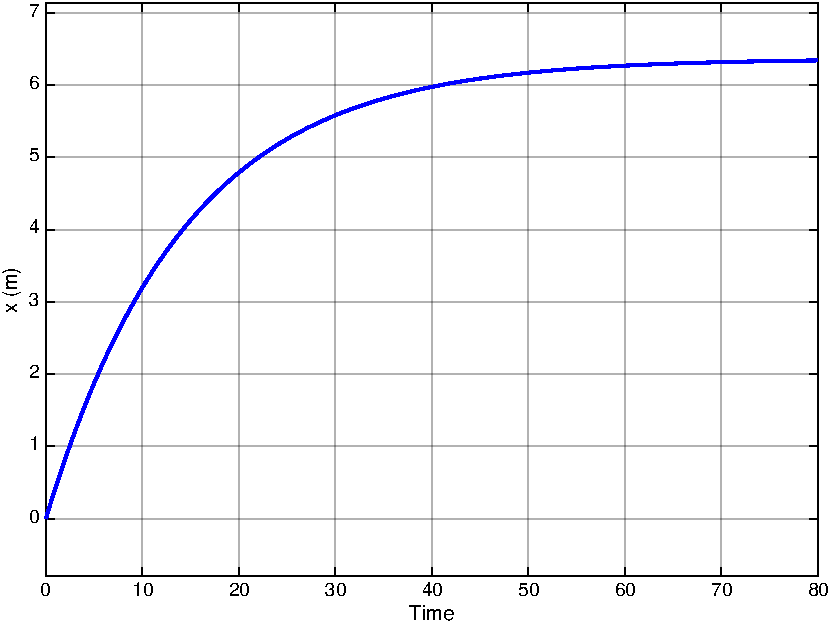
\includegraphics[width=\linewidth]{phan_tich_x_dirac.pdf}
            \caption{$x$}
        \end{subfigure}\hfill
        \begin{subfigure}[b]{0.495\linewidth}
            \centering
            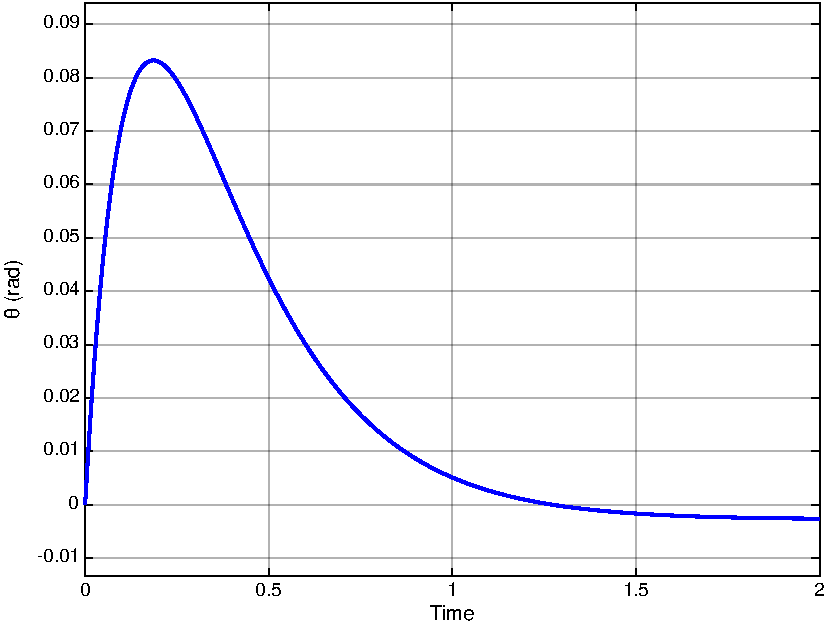
\includegraphics[width=\linewidth]{phan_tich_theta_dirac.pdf}
            \caption{$\theta$}
        \end{subfigure}
        \caption{Kết quả mô phỏng với đầu vào là hàm Dirac}
    \end{figure}
    \item \textbf{Phân tích, nhận xét}
    \begin{itemize}
        \item 
    \end{itemize}
\end{itemize}


\subsubsection{Đầu vào hàm nấc đơn vị}
\begin{itemize}
    \item Kết quả mô phỏng 
    \begin{figure}[ht]
        \centering
        \begin{subfigure}[b]{0.495\linewidth}
            \centering
            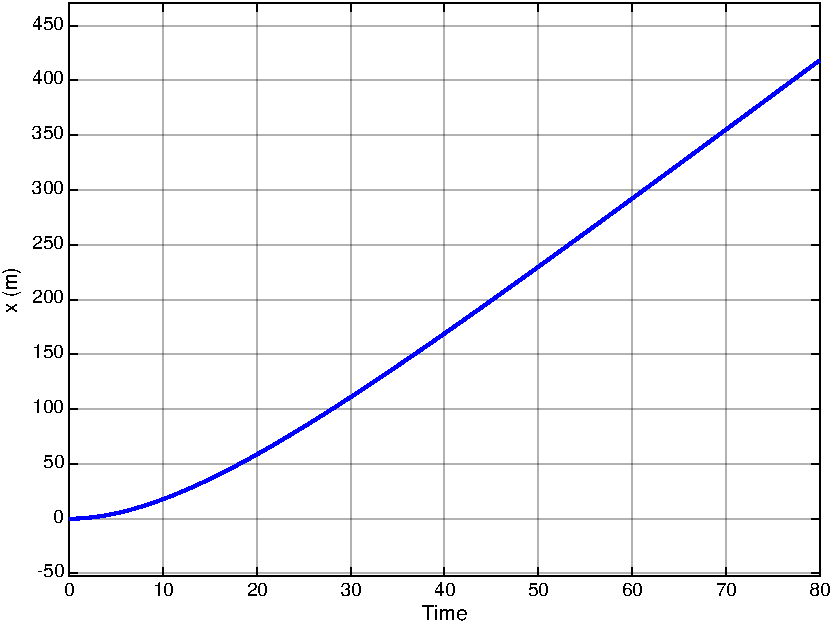
\includegraphics[width=\linewidth]{phan_tich_x_step.pdf}
            \caption{$x$}
        \end{subfigure}\hfill
        \begin{subfigure}[b]{0.495\linewidth}
            \centering
            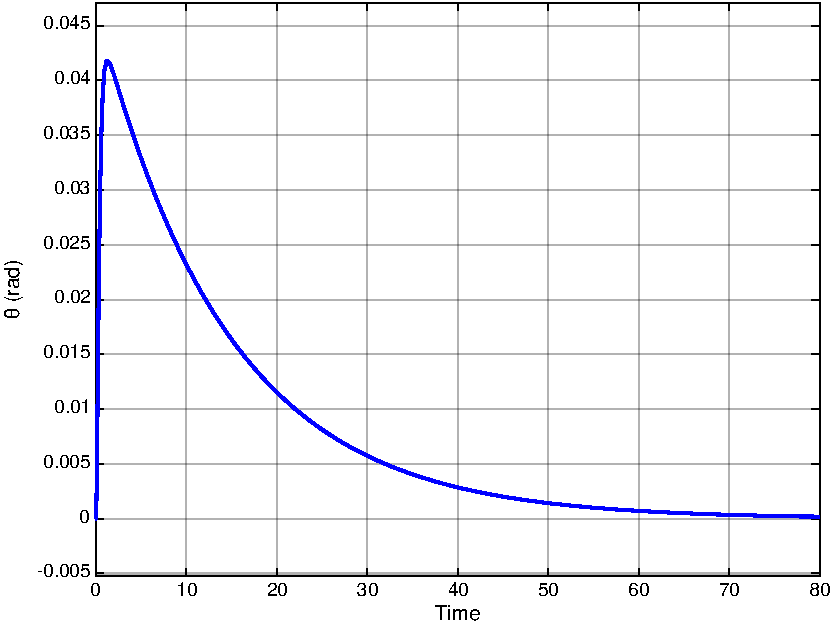
\includegraphics[width=\linewidth]{phan_tich_theta_step.pdf}
            \caption{$\theta$}
        \end{subfigure}
        \caption{Kết quả mô phỏng với đầu vào là hàm nấc đơn vị}
    \end{figure}
    \item \textbf{Phân tích, nhận xét}
    \begin{itemize}
        \item 
    \end{itemize}
\end{itemize}


\subsubsection{Đầu vào hàm \eqref{eqn:hxd}}
\begin{itemize}
    \item Kết quả mô phỏng 
    \begin{figure}[ht]
        \centering
        \begin{subfigure}[b]{0.495\linewidth}
            \centering
            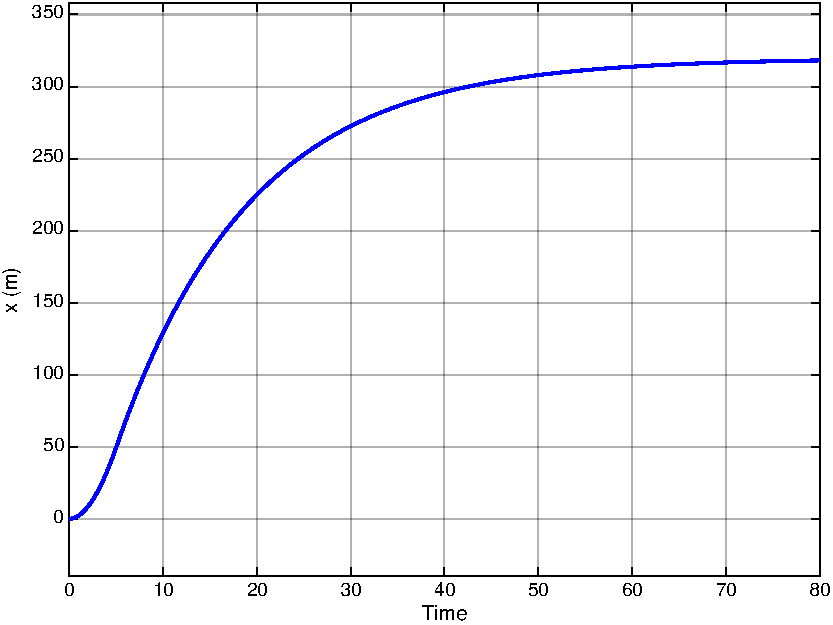
\includegraphics[width=\linewidth]{phan_tich_x_f.pdf}
            \caption{$x$}
        \end{subfigure}\hfill
        \begin{subfigure}[b]{0.495\linewidth}
            \centering
            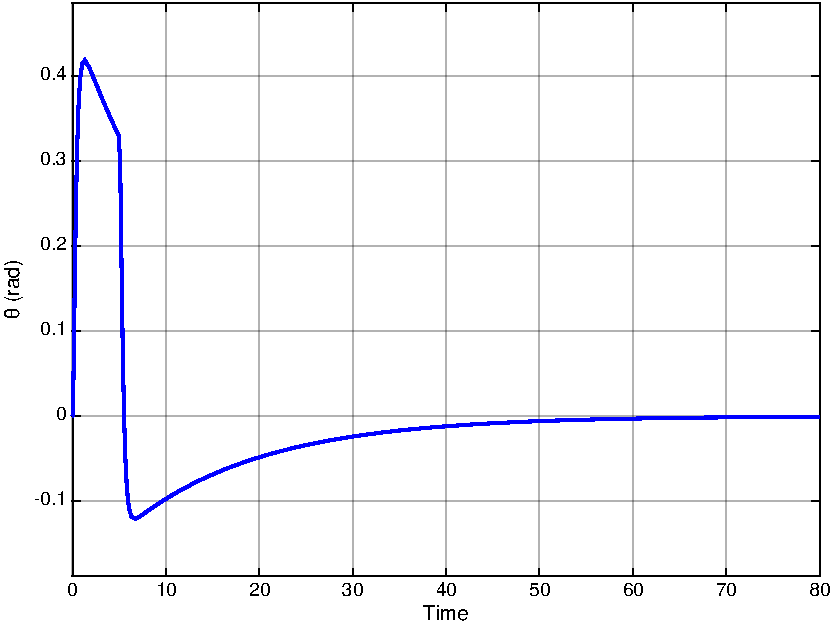
\includegraphics[width=\linewidth]{phan_tich_theta_f.pdf}
            \caption{$\theta$}
        \end{subfigure}
        \caption{Kết quả mô phỏng với đầu vào là hàm \eqref{eqn:hxd}}
    \end{figure}
    \item \textbf{Phân tích, nhận xét}
    \begin{itemize}
        \item 
    \end{itemize}
\end{itemize}

\section{Thiết kế hệ thống điều khiển}
\subsection{Thiết kế bộ điều khiển PID cho góc con lắc}
\subsubsection{Yêu cầu thiết kế}
\begin{minipage}[t]{0.3\linewidth}
    \textbf{Đề bài}
\end{minipage}\begin{minipage}[t]{0.6\linewidth}
    \begin{itemize}
        \item Giữ cho con lắc ở vị trí thẳng đứng sau khi bị xô lệch. 
    \end{itemize}
\end{minipage}

\vspace{\baselineskip}

\begin{minipage}[t]{0.3\linewidth}
    \textbf{Yêu cầu thiết kế}
\end{minipage}\begin{minipage}[t]{0.6\linewidth}
    \begin{itemize}[noitemsep,topsep=0pt]
        \item Thời gian xác lập của góc lệch $\theta$ phải nhỏ hơn 5 giây.
        \item Góc lệch của con lắc không được vượt quá 0.05 radian so với vị trí thẳng đứng.
    \end{itemize}
\end{minipage}

\vspace{\baselineskip}

\begin{minipage}[t]{0.3\linewidth}
    \textbf{Phương pháp thực hiện}
\end{minipage}\begin{minipage}[t]{0.6\linewidth}
    \begin{itemize}[noitemsep,topsep=0pt]
        \item Sử dụng phương pháp quỹ đạo nghiệm số để xác định các thông số của bộ điều khiển PID.
        \item Mô phỏng tác động của một xung đơn vị vào xe đẩy, sau đó quan sát quá trình con lắc quay trở lại vị trí thẳng đứng.
        \item Đưa ra nhận xét và đánh giá đáp ứng của góc lắc.
    \end{itemize}
\end{minipage}

\subsubsection{Thiết kế bộ điều khiển}

Sử dụng công cụ \textbf{Control System Designer} của MATLAB để thiết kế bộ điều khiển. 
\begin{lstlisting}[style=matlabstyle,caption=Thiết kế bộ điều khiển PID cho hàm truyền $G_2(s)$]
controlSystemDesigner('rlocus', G2);
\end{lstlisting}

Do bộ điều khiển PID có một cực tại $s=0$ và 2 zero nên trong cửa sổ \textbf{Control System Designer}, nhóm chọn 2 zero phức (complex zero). 
\begin{align}
    C(s) = K_p + \frac{K_i}{s} + K_ds = \frac{K_ds^2 + K_ps +K_i}{s}
\end{align}

\begin{center}
    \captionsetup{type=figure}
    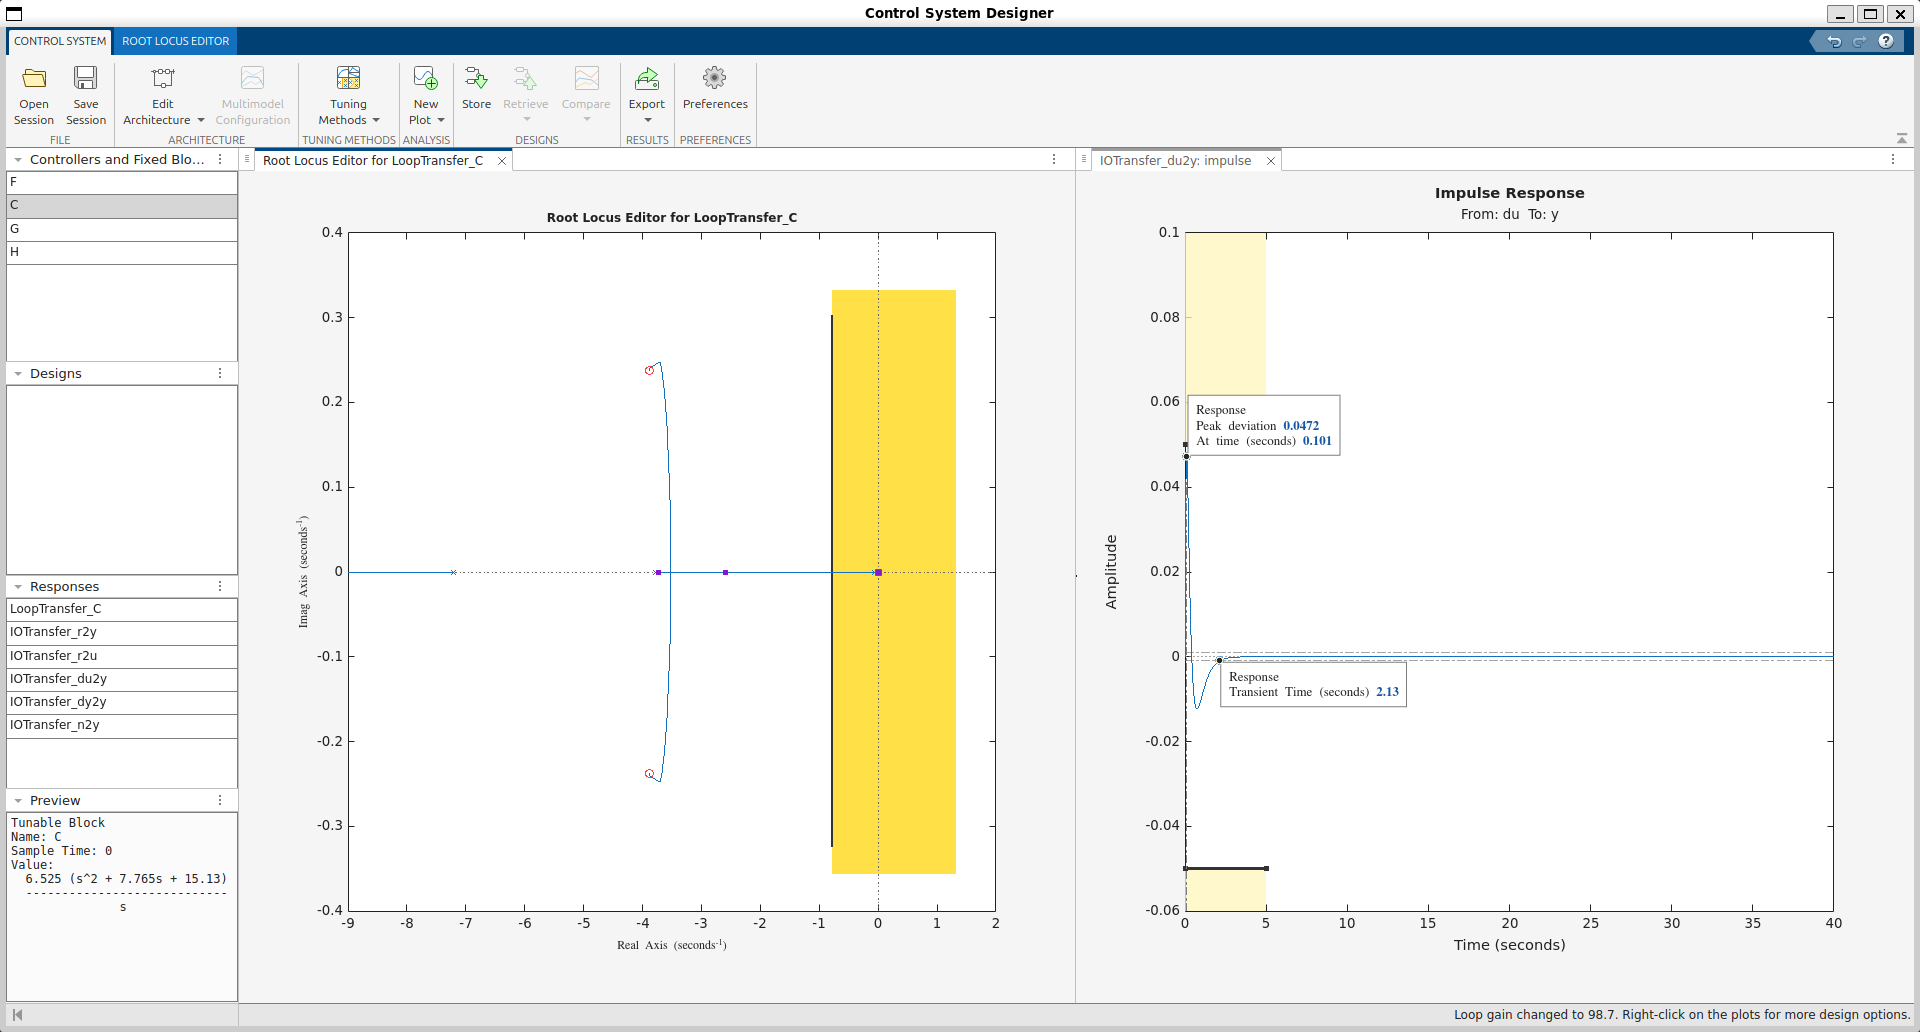
\includegraphics[width=\linewidth]{thiet_ke_PID_con_lac.png}
    \caption{Thiết kế bộ điều khiển PID cho góc lắc $\theta$ con lắc}
\end{center}

Vùng màu vàng trong \textbf{Root Locus Editor for LoopTransfer\_C} và  \textbf{Impulse Response} là các vùng mà không thỏa mãn yêu cầu đề bài. Bằng cách kéo thả cặp zero phức của bộ điều khiển và các cực của hệ kín (hình vuông màu tím) ở bên cửa sổ \textbf{Root Locus Editor for LoopTransfer\_C} vào vùng màu trắng, nhóm tìm được hàm truyền của bộ điều khiển PID cho góc lắc $\theta$ của con lắc.
\begin{align}
    C_{\text{PID con lắc}} = \frac{6.525 (s^2 + 7.765s + 15.13)}{s}
\end{align}

Các hệ số của bộ điều khiển PID con lắc là
\begin{itemize}
    \item $K_p = 50.6646$.
    \item $K_i = 98.7160$.
    \item $K_d = 6.5250$.
\end{itemize}


\subsubsection{Mô phỏng bằng MATLAB/Simulink}

Dưới đây là sơ đồ MATLAB/Simulink cho hệ thống điều khiển con lắc:
\newpage
\begin{figure}[ht]
    \centering
    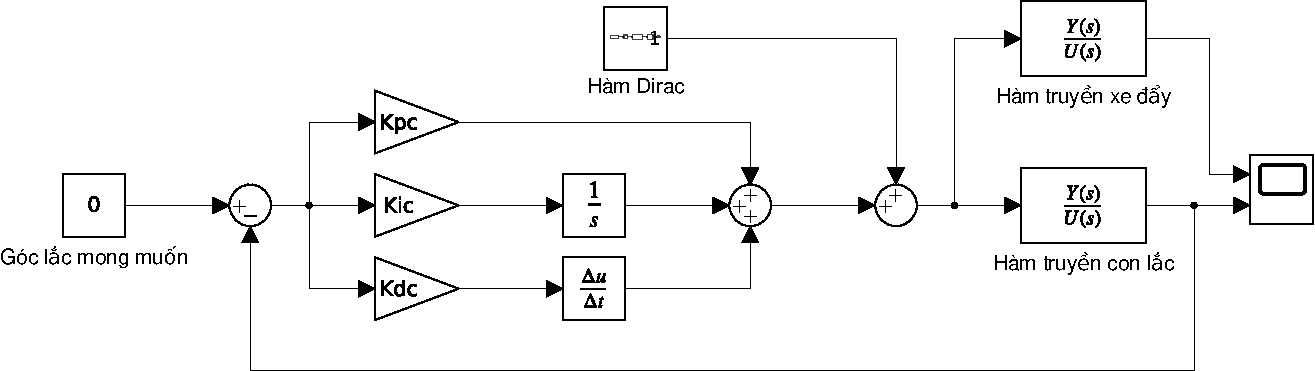
\includegraphics[width=\linewidth]{MATLAB_4.pdf}
    \caption{Sơ đồ MATLAB/Simulink cho hệ thống điều khiển con lắc}
\end{figure}

Kết quả mô phỏng bằng MATLAB/Simulink
\begin{figure}[ht]
    \centering
    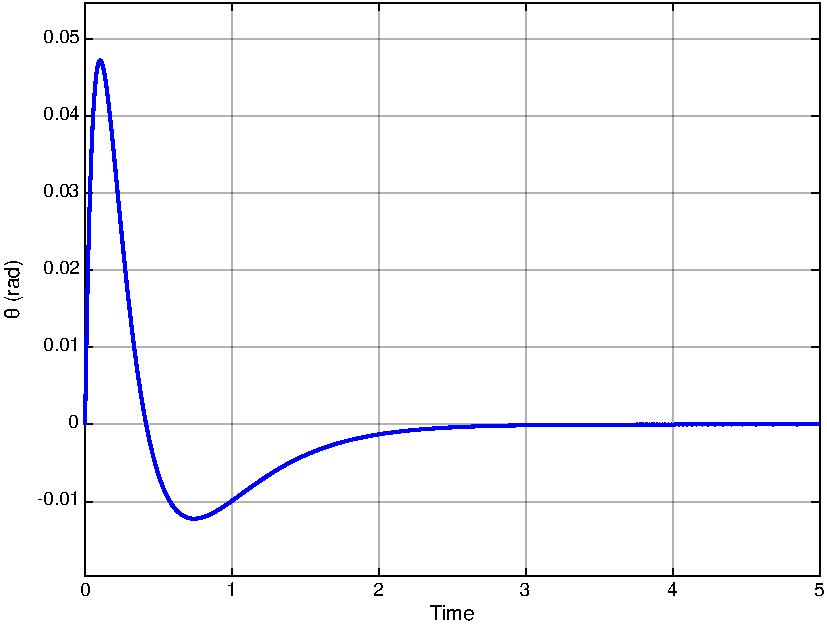
\includegraphics[width=\linewidth]{MATLAB_5.pdf}
    \caption{Kết quả mô phỏng bằng MATLAB/Simulink cho hệ thống điều khiển con lắc}
\end{figure}

\subsubsection{Đánh giá, nhận xét}


\subsection{Thiết kế bộ điều khiển PID cho vị trí xe đẩy}
\subsubsection{Yêu cầu thiết kế}
\begin{minipage}[t]{0.3\linewidth}
    \textbf{Đề bài}
\end{minipage}\begin{minipage}[t]{0.6\linewidth}
    \begin{itemize}
        \item  Di chuyển xe đẩy đến vị trí mong muốn.
    \end{itemize}
\end{minipage}

\vspace{\baselineskip}

\begin{minipage}[t]{0.3\linewidth}
    \textbf{Yêu cầu thiết kế}
\end{minipage}\begin{minipage}[t]{0.6\linewidth}
    \begin{itemize}[noitemsep,topsep=0pt]
        \item Thời gian xác lập cho $x$ nhỏ hơn 3 giây.
        \item Độ vọt lố nhỏ 15\%.
    \end{itemize}
\end{minipage}

\vspace{\baselineskip}

\begin{minipage}[t]{0.3\linewidth}
    \textbf{Phương pháp thực hiện}
\end{minipage}\begin{minipage}[t]{0.6\linewidth}
    \begin{itemize}[noitemsep,topsep=0pt]
        \item Sử dụng phương pháp quỹ đạo nghiệm số để xác định thông số cho bộ điều khiển PID.
        \item Mô phỏng đáp ứng hệ thống với vị trí mong muốn $x_d = 0.5$ m.
        \item Nhận xét và đánh giá cả đáp ứng của góc lắc và vị trí xe đẩy.
    \end{itemize}
\end{minipage}

\subsubsection{Thiết kế bộ điều khiển}

Sử dụng công cụ \textbf{Control System Designer} của MATLAB để thiết kế bộ điều khiển. 
\begin{lstlisting}[style=matlabstyle,caption=Thiết kế bộ điều khiển PID cho hàm truyền $G_2(s)$]
controlSystemDesigner('rlocus', G1);
\end{lstlisting}


\begin{center}
    \captionsetup{type=figure}
    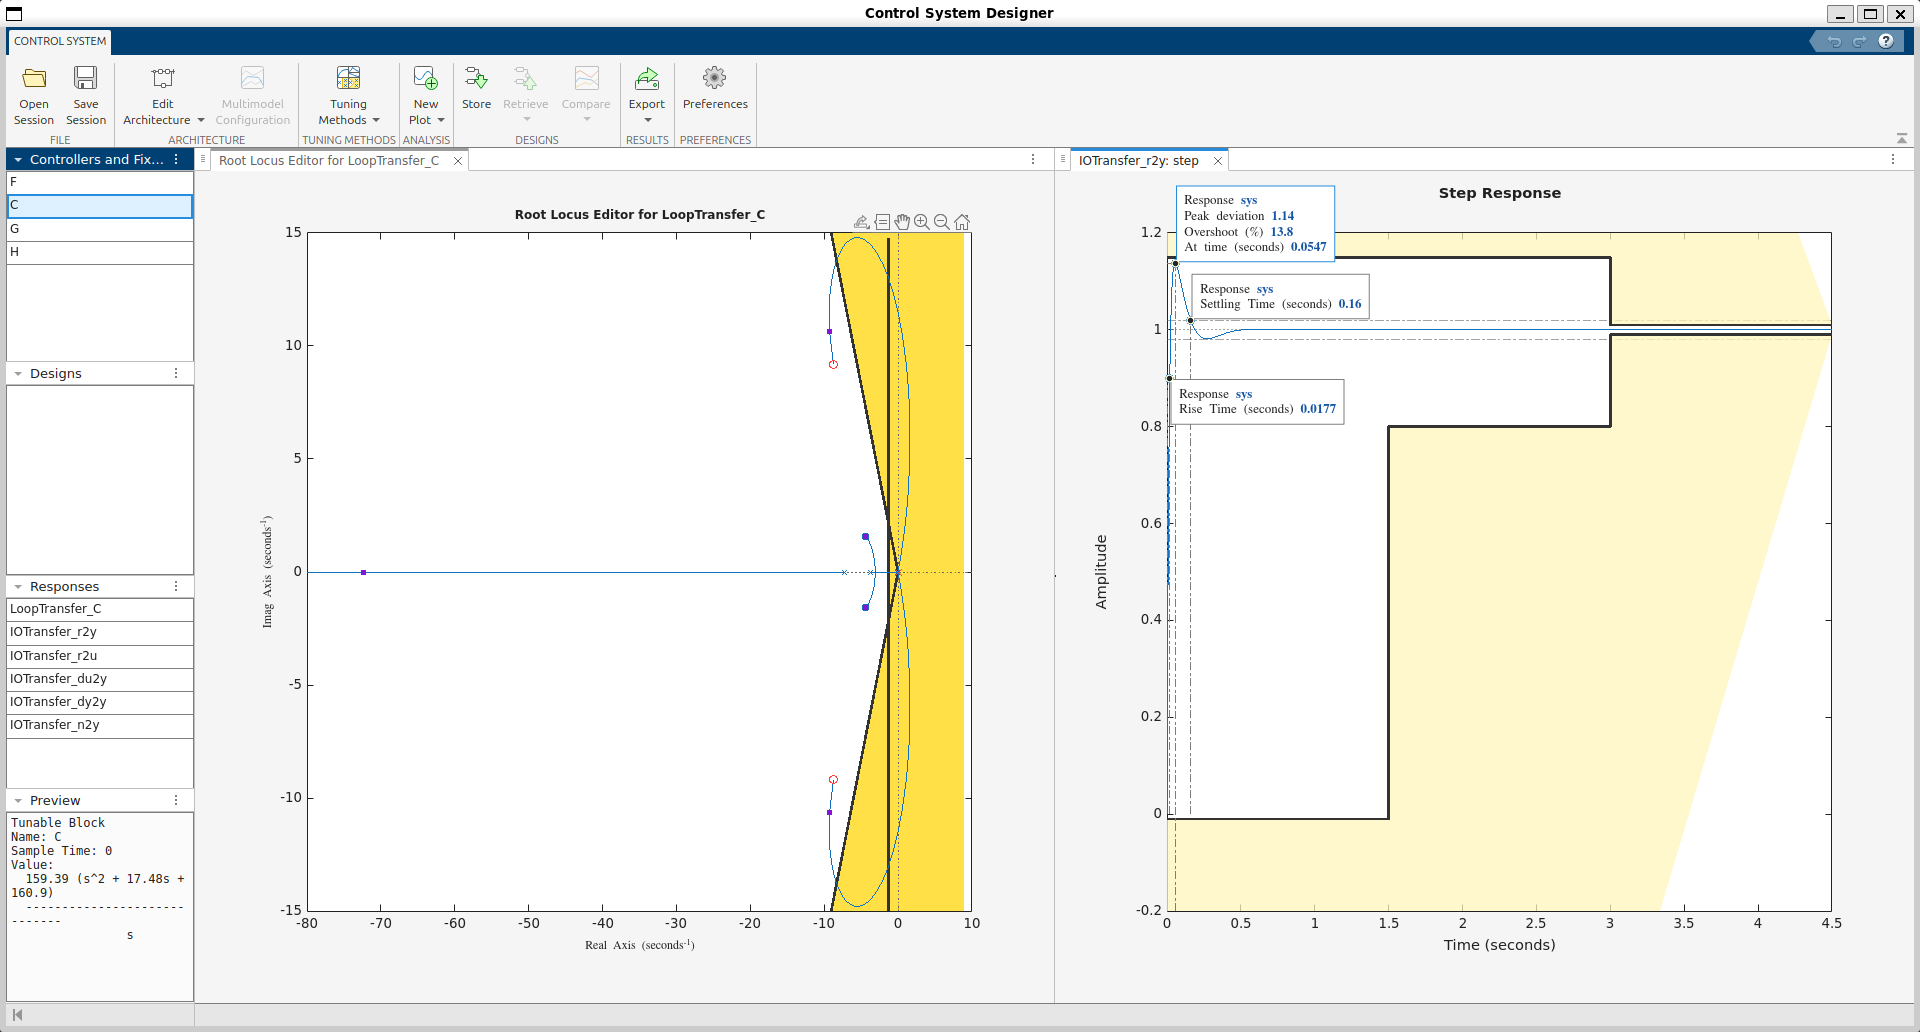
\includegraphics[width=\linewidth]{thiet_ke_PID_xe_day.png}
    \caption{Thiết kế bộ điều khiển PID cho vị trí $x$ xe đẩy}
\end{center}

Vùng màu vàng trong \textbf{Root Locus Editor for LoopTransfer\_C} và  \textbf{Step Response} là các vùng mà không thỏa mãn yêu cầu đề bài. Bằng cách kéo thả cặp zero phức của bộ điều khiển và các cực của hệ kín (hình vuông màu tím) ở bên cửa sổ \textbf{Root Locus Editor for LoopTransfer\_C} vào vùng màu trắng, nhóm tìm được hàm truyền của bộ điều khiển PID cho vị trí $x$ xe đẩy.
\begin{align}
    C_{\text{PID xe đẩy}} = \frac{159.4 s^2 + 2786 s + 2.564\cdot 10^4}{s}
\end{align}

Các hệ số của bộ điều khiển PID xe đẩy là
\begin{itemize}
    \item $K_p = 2786.3$.
    \item $K_i = 2.5638\cdot 10^4$.
    \item $K_d = 159.3864 $.
\end{itemize}

\subsubsection{Mô phỏng bằng MATLAB/Simulink}

Dưới đây là sơ đồ MATLAB/Simulink cho hệ thống điều khiển xe đẩy:
\newpage
\begin{figure}[ht]
    \centering
    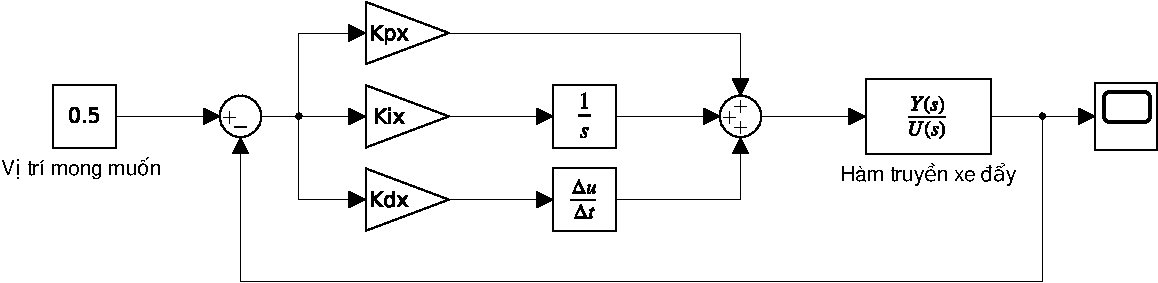
\includegraphics[width=\linewidth]{MATLAB_7.pdf}
    \caption{Sơ đồ MATLAB/Simulink cho hệ thống điều khiển xe đẩy}
\end{figure}

Kết quả mô phỏng bằng MATLAB/Simulink
\begin{figure}[ht]
    \centering
    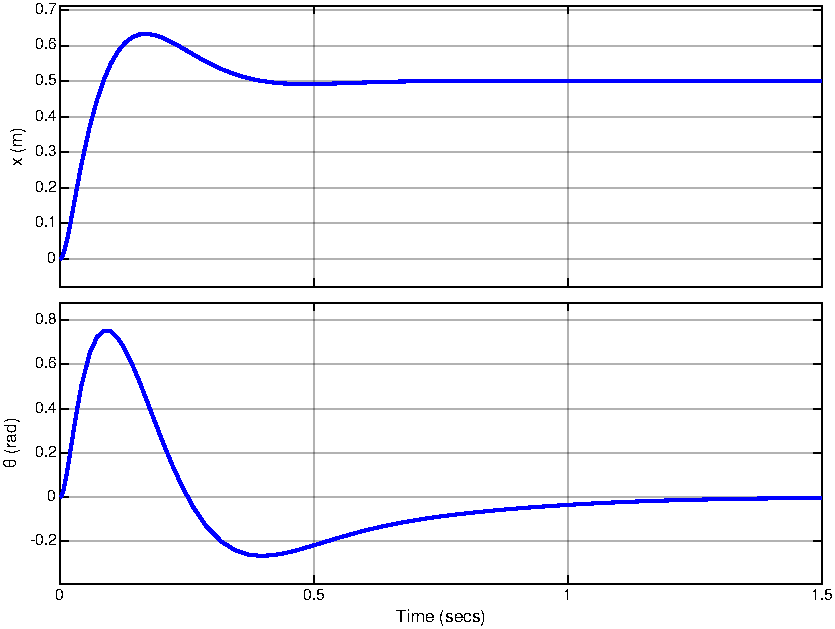
\includegraphics[width=\linewidth]{MATLAB_6.pdf}
    \caption{Kết quả mô phỏng bằng MATLAB/Simulink cho hệ thống điều khiển xe đẩy}
\end{figure}
\subsubsection{Đánh giá, nhận xét}

\subsection{Thiết kế bộ điều khiển không gian trạng thái}
\subsubsection{Yêu cầu thiết kế}
\begin{minipage}[t]{0.3\linewidth}
    \textbf{Đề bài}
\end{minipage}\begin{minipage}[t]{0.6\linewidth}
    \begin{itemize}
        \item Điều khiển cả góc con lắc $\theta$ và vị trí xe đẩy $x$.
    \end{itemize}
\end{minipage}

\vspace{\baselineskip}

\begin{minipage}[t]{0.3\linewidth}
    \textbf{Yêu cầu thiết kế}
\end{minipage}\begin{minipage}[t]{0.6\linewidth}
    \begin{itemize}[noitemsep,topsep=0pt]
        \item Thời gian xác lập cho $x$ và $\theta$ nhỏ hơn 5 giây.
        \item Thời gian tăng cho $x$ nhỏ hơn 0.5 giây. 
        \item Độ vột lố tối đa cho $\theta$ nhỏ hơn 0.35 radian (20$^\circ$). 
        \item Sai số xác lập nhỏ hơn 2\% cho cả $x$ và $\theta$. 
    \end{itemize}
\end{minipage}

\vspace{\baselineskip}

\begin{minipage}[t]{0.3\linewidth}
    \textbf{Phương pháp thực hiện}
\end{minipage}\begin{minipage}[t]{0.6\linewidth}
    \begin{itemize}[noitemsep,topsep=0pt]
        \item Thiết kế bộ điều khiển không gian trạng thái theo phương pháp đặt cực để đạt được độ ổn định cho cả vị trí và góc. 
        \item Đánh giá bộ điều khiển thông qua mô phỏng MATLAB/Simulink. 
    \end{itemize}
\end{minipage}


\newpage
Au point que j’expirais, tu m’as rendu le jour\\
Baiser, dont jusqu’au coeur le sentiment me touche,\\
Enfant délicieux de la plus belle bouche\\
Qui jamais prononça les Oracles d’Amour.\\

Mais tout mon sang s’altère, une brûlante fièvre\\
Me ravit la couleur et m’ôte la raison ;\\
Cieux ! j’ai pris à la fois sur cette belle lèvre\\
D’un céleste Nectar et d’un mortel poison.\\

Ah ! mon Ame s’envole en ce transport de joie !\\
Ce gage de salut, dans la tombe m’envoie ;\\
C’est fait ! je n’en puis plus, Élise je me meurs.\\

Ce baiser est un sceau par qui ma vie est close :\\
Et comme on peut trouver un serpent sous des fleurs,\\
J’ai rencontré ma mort sur un bouton de rose.\\

\end{document}